\documentclass[11pt,titlepage]{article}
\input{\string~/.macros}
\usepackage[a4paper, total={6.5in, 9in}]{geometry}   % margin=1in
\usepackage[utf8]{inputenc}
\usepackage{caption}
\usepackage{subcaption}
\usepackage{titlepic}
\usepackage{graphicx}
\graphicspath{{../data/imgs/}}
\usepackage{hyperref}
\hypersetup{colorlinks=true, linktoc=all, linkcolor=blue, citecolor=blue}
\usepackage[backend=biber,sorting=none]{biblatex}
\addbibresource{references.bib}
\setcounter{MaxMatrixCols}{20}

% \linespread{1.5}
 
\newcommand{\heading}[1]{(#1)}
\newcommand{\bheading}[1]{\textbf{(#1)}}

\newcommand{\bsigma}{\boldsymbol{\sigma}}
\newcommand{\bepsilon}{\boldsymbol{\varepsilon}}
\renewcommand{\epsilon}{\varepsilon}
\renewcommand{\bf}{\mathbf{f}}
\newcommand{\ta}{\tilde{a}}
\renewcommand{\bphi}{\boldsymbol{\varphi}}

\title{Linear Elasticity Simulation for Stress Visualization}
\author{Peiqi Wang, Eris Zhang}
\titlepic{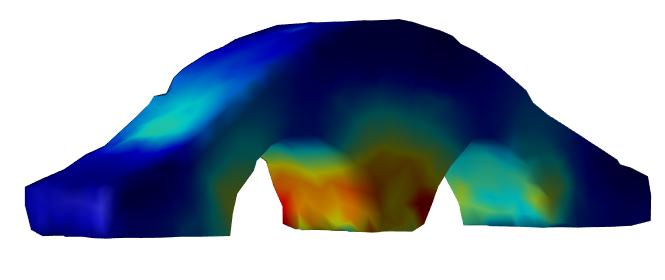
\includegraphics[width=3in]{goldstandard_vm/resized/archbridge_tiny_goldstandard}}
\date{April 10, 2019}

\begin{document}

\maketitle
\tableofcontents

\newpage
\section{Introduction}

In computational fabrication, it is crucial to quantify how a 3D printed objects might break or fail using linear elasticity simulations.~\cite{zhou_panetta_zorin_2013}~\cite{langlois_shamir_dror_matusik_levin_2016}~\cite{langlois_shamir_dror_matusik_levin_2016} To enable interactive design and optimization of shapes such that failure cases are minimized, there has been work to increase the speed of simulation with novel interpolation algorithms~\cite{schulz_xu_zhu_zheng_grinspun_matusik_2017} or with the help of modern parallel hardwares.~\cite{dick_georgii_westermann_2011}. A particularly interesting and relevant work uses matrix-free iterative methods to perform real time simulation on GPU.~\cite{yadav_suresh_2014}~\cite{marix_free_voxel_fem_thesis_2018}

% There is recent interest in utilizing iterative methods  line of work uses iterative methods to solve linear elasticity systems.~\cite{multigrid_preconditioning_thesis_2016}

 
The aim of this report is to explore potential methods to visualize failure cases, i.e. fractures, breakage, etc. for solid shapes of elastic material in real time. For our use case, precision of simulation is only important up to the visualization not deviating from the ground truth by human perception. To exploit this assumption, we explored different iterative methods to solve the linear system resulted from finite element discretization. We explored linear basis functions on both tetrahedron element and regular hexahedron element. In the latter case, we can avoid the costly operation of numerically computing integrals at each element, which opens up opportunity to use matrix-free iterative method with substantial reduction in memory and time cost.


\section{Linear Elasticity}

\subsection{Background}

Continuum mechanics deals with behavior of material modeled as a continuous mass. The study of elastic material is a subset of continuum mechanics that models the ability of a material to resist influence and return to its original configuration when the influence is removed. The following definitions are important to elasticity theory and provide important background for rest of the report.~\cite{bauchau_craig_2009}

\begin{enumerate}
    \item \bheading{stress} describes internal force over a differential area at a point, which can be represented as a symmetric second order tensor $\bsigma$,
    \[
        \bsigma = 
        \begin{bmatrix}
            \sigma_{11} & \sigma_{12} & \sigma_{13} \\
            \sigma_{21} & \sigma_{22} & \sigma_{23} \\
            \sigma_{31} & \sigma_{32} & \sigma_{33} \\
        \end{bmatrix}    
    \]
    where
    \[
        \sigma_{ij} = \lim_{dA_i \to 0} \dfrac{F_j}{dA_i}
    \] 
    represents force applied in $j$-th coordinate axis over a differential plane orthogonal to $i$-th coordinate axis. 
    \item \bheading{strain} describes deformation by relative displacements, which can be represented as a symmetric second order tensor $\bepsilon$,
    \[
        \bepsilon = 
        \begin{bmatrix}
            \epsilon_{11} & \epsilon_{12} & \epsilon_{13} \\
            \epsilon_{21} & \epsilon_{22} & \epsilon_{23} \\
            \epsilon_{31} & \epsilon_{32} & \epsilon_{33} \\
        \end{bmatrix}
    \]
    where $\epsilon_{ii}$ are axial strains and $\epsilon_{ij}$ where $i\neq j$ are shearing strains.
    \item \bheading{displacement} describes how much a point moves from referenced to deformed configuration, which can be represented as component-wise displacement, $\bu$
    \[
        \bu = \p{u_1, u_2, u_3}
    \]
    \item \bheading{yield} a point on a stress-strain curve of a material that indicates the limit of elastic behavior. Material experiencing stress over the yield point will suffer from permanent deformations.
    \item \bheading{von Mises yielding criterion} Ultimately, we are interested in computing the stress field over all points within a solid geometry, from which we can deduce material yielding by comparing the effective stress $\sigma_e$ with material-specific yield stress $\sigma_y$. Simply, we use Von Mises' criterion to determine yielding, 
    \[
        \sigma_e = \frac{1}{\sqrt{2}}\sqrt{
            (\sigma_{11} - \sigma_{22})^2 
            + (\sigma_{22} - \sigma_{33})^2 
            + (\sigma_{33} - \sigma_{11})^2
            + 6(\sigma_{23}^2 + \sigma_{31}^2 + \sigma_{12}^2)
        } > \sigma_y
    \]
\end{enumerate}


\subsection{Problem Assumptions}

Here, we lay down simplifying assumptions for our problem.
\begin{enumerate}
    \item \bheading{Analytic stress/strain} If we assume that stress and strain field is analytic in small neighborhood of a point, we can guarantee convergent Taylor series expansion, which leads to simplier formulation of differential equation governing materials' elastic behavior. This assumption, for example, helped with derivation of Green-Lagrangian strain tensor
    \[
        \epsilon_{ij} = \p{u_{i,j} + u_{j,i} - u_{k,i}u_{k,j}}    
    \]
    \item \bheading{Small deformations} Typically, elastic material exhibit a nonlinear relationship between stress and strain. However, if we assume for small deformation only, stress-strain is linear, hence the name \textit{linear} elasticity. We can employ Hooke's law to model the relationship between stress and strain.
    \[
        \bsigma = \bC : \bepsilon
    \]
    where $\bC$ is a fourth-order stiffness tensor.
    \item \bheading{Isotropic homogeneous material} Typically, material exhibit direction or location specific behavior. If materials are characterized by properties independent of orientation and coordinate system, we can reduce the number of material-dependent constants to 2 (i.e. $\lambda,\mu$),
    \[
        \bsigma = \bC : \bepsilon
        \quad \quad \rightarrow \quad \quad
        \bsigma = 2\mu\bepsilon + \lambda \tr{\bepsilon} \bI
    \]
    Also note that the stiffness tensor is symmetric, i.e. $\bC_{ijkl} = \bC_{klij}$. This is true even for anisotropic materials.
    \item \bheading{Static equilibrium} We are only interested in modeling static objects. With this assumption, we obtain a simpler formula from Newton's second law on conservation of linear and angular momentum.
    \[
        \nabla\cdot\bsigma + \bf = \rho \ddot{\bu}
        \quad \quad \rightarrow \quad \quad
        \nabla\cdot\bsigma + \bf = 0
    \]
    where $\bf$ are body forces, and $\rho$ is density of the material.
\end{enumerate}


\subsection{Differential Equations}

From physical laws and simplifying assumptions, we can derive a set of equations governing linear elasticity with respect to the stress field $\bsigma$, the strain field $\bepsilon$, and the displacement field $\bu$. We express the equations in tensor notations.
\begin{enumerate}
    \item \bheading{Equilibrium Equations} express equilibirum condition imposed to the stress field by Newton's second law
    \[
        \nabla\cdot\bsigma + \bf = 0
        \quad\quad\quad\quad
        \sigma_{ji,j} + f_i = 0
    \]
    \item \bheading{Kinematics Equations} express deformation with respect to displacement without reference to forces that created them. 
    \[
        \bepsilon = \dfrac{1}{2} \p{
            \nabla \bu + \nabla\bu^T
        }
        \quad\quad\quad\quad
        \epsilon_{ij} = 
            \frac{1}{2} \p{
                u_{i,j} + u_{j,i}
            }
            % \frac{1}{2} \p{
            %     \frac{\partial u_i}{\partial x_j} + \frac{\partial u_j}{\partial x_i}}
    \]
    \item \bheading{Constitutive Law} describes behavior of material under stress. We approximate behavior of linear elastic material with Hooke's Law
    \[
        \bsigma = \bC : \bepsilon
        \quad\quad\quad\quad
        \sigma_{ij} = C_{ijkl} \epsilon_{kl}
    \]
    where $\bC$ is a 4-th order stiffness tensor encoding material properties. Specifically, under the assumption of isotropic material, the relationship is simplified to 
    \[
        \bsigma = 2\mu\bepsilon + \lambda \tr{\bepsilon} \bI
        \quad\quad\quad\quad
        \sigma_{ij} = 2\mu \epsilon_{ij} + \lambda \epsilon_{kk} \delta_{ij}
    \]
    where $\lambda,\mu$ are Lam\'{e}'s first and second parameter can be written as material-specific constants - Poisson's ratio $\nu$ and Young's modulus $E$,
    \[
        \mu = \frac{E}{2(1+\nu)}
        \quad\quad\quad\quad
        \lambda = \frac{E\nu}{(1+\nu)(1-2\nu)}
    \]
\end{enumerate}


\subsection{Boundary Value Problem}
For our purposes, it is easier to eliminate stress and strain to seek a set of equations where the displacement field is the primary unknown. We can achieve this by writing the strain $\bsigma$ in the equilibrium equation as a function of displacement $\bu$ using the constitutive law and kinematics equations. In other words, we seek displacement field $\bu$ in $\R^3$ satisfying
\begin{align*}
    -\nabla \cdot \bC \p{\bepsilon(\bu)}
        &= \bf & \bx\in\Omega \\
    \bu &= 0   &\bx\in\Gamma
\end{align*}
where $\Omega\in\R^3$ is a closed and bounded region occupied by a linear elastic solid, with boundary $\partial\Omega$. $\Gamma \subset \partial\Omega$ is part of boundary that the object cannot be displaced. $\sV := \pc{\bv\in H(\Omega,\R^3) \mid \bv|_{\Gamma} = \mathbf{0}}$ is a first Sobolev space satisfying the zero boundary condition on $\Gamma$. $\bepsilon$ is a linear differential operator over the displacement field $\bu$, while $\bC$ is a linear operator over the the strain field $\bepsilon(\bu)$, which is positive definite for linear elastic isotropic material. It is easy to see that $\sL := -\nabla \cdot \p{\bC \bepsilon(\cdot)}$ is a linear differential operator. 

\section{Finite Elements}
It is conventional to use finite element method to solve linear elasticity equations for 3-dimensional objects with complex geometry. We will formulate the boundary value problem in both the weak and variational form. The two formulations are equivalent in our setup. We will then discuss computer implementation strategies on tetrahedron elements, and briefly on regular hexahedron elements.

\subsection{Weak Form}
The goal is to estimate $\bu$ in a finite dimensional function space $\sV_m\subset\sV$ spanned by a set of basis functions $\pc{\bu_1, \cdots, \bu_m} \subset \sV$. We can formulate linear elasticity weakly as
\[
    \int_{\Omega} \bC\bepsilon(\bu) : \bepsilon(\bv) d\bx
    = 
    \int_{\Omega} \bf \cdot \bu d\bx
\]
for all $\bv \in\sV$. The left hand side is obtained via Green's first identity assuming a pure displacement formulation with no traction force on the boundary.~\cite{multigrid_preconditioning_thesis_2016} We can define a bilinear form $\ta(\cdot,\cdot)$
\[
    \ta(\bu,\bv) = \inner{\sL \bu}{\bv}
        = \int_{\Omega} \bC \bepsilon(\bu) : \bepsilon(\bv) d\bx    
\]
where $\inner{\cdot}{\cdot}$ is $L^2$ norm over $\Omega$. 


\subsection{Variational Form}
By theorem 9.1 in~\cite{iserles_2009} and the following proposition, $\sL \bu = \bf$ is the Euler-Lagrange equation of following variational problem
\[
    \sJ(\bu) := \ta(\bu,\bu) - 2\inner{\bf}{\bu}
\]
where $\sJ: \sV\to \R$ is a functional and $\bu\in\sV$. The theorem also guarantees the uniqueness and existence of solution for the boundary value problem. Therefore, we can solve for an equivalent optimization problem
\[
    \min_{\bu\in \sV} \;\; \sJ(\bu)
    \quad \text{ where } \quad
    \sJ(\bu) = 
        \underbrace{\frac{1}{2}\int_{\Omega} \bC \bepsilon(\bu) : \bepsilon(\bu) d\bx }_\text{potential energy}
      - \underbrace{\int_{\Omega} \bf \cdot\bu d\bx}_\text{work}
\]
This amounts to applying the principle of least work to mechanical systems. Simply, we are minimizing the internal potential energy and work done by external force (e.g. gravity) on the object. 

\subsection{Discretization}

There are many ways to discretize the domain. We will clarify computer implementations on tetrahedron elements first, and then briefly explain how we can adapt similar strategies for regular hexahedron elements. We construct a mesh $\sT$ that partitions the domain $\Omega$ where each $\Omega^e \in\sT$ is a tetrahedron and $n$ is number of vertices of the mesh. We define a linear nodal basis function that is 0 at all vertices of the mesh, except has value of 1 at one vertex . Note the boundary value equations are vector valued, so we compose the same scalar valued nodal basis function for each component of the vector field. Therefore, we arrive at $3n$ linear basis that form a finite dimensional subspace of $\sV$,
\[
    \sV_{3n} = \text{span} \pc{
        \varphi_1, \cdots, \varphi_{3n}
    }
\]
The variational formulation over the discretized domain is then as follows,
\[
    \min_{ \bd\in \R^{3n}} \;\; \sJ_{3n}(\bd)
        \quad\text{ where }\quad
        \sJ_{3n}(\bd) := \sJ(\bu) = 
        \sum_{\Omega^e \in \sT} \pb{
            \frac{1}{2}\int_{\Omega^e} \bC \bepsilon(\bu) : \bepsilon(\bu) d\bx 
            - \int_{\Omega^e} \bf \cdot\bu d\bx
        }
\]
where $\bd\in\R^{3n}$ are coefficients to linear nodal basis functions and could be interpreted as displacements in 3 coordinate directions at each vertex of the mesh. The displacement field $\bu$ and coefficient $\bd$ are related as follows in the above equation,
\[
    \bu = 
    \begin{pmatrix}
        \sum_{i=1}^n \xi_i \varphi_i \\
        \sum_{i=1}^n \eta_i \varphi_i \\
        \sum_{i=1}^n \zeta_i \varphi_i \\
    \end{pmatrix}
    =
    \begin{bmatrix}
        \varphi_1 & 0 & 0 & \varphi_2 & 0 & 0 & \cdots & \varphi_{n} & 0 & 0 \\
        0 & \varphi_1 & 0 & 0 & \varphi_2 & 0 & \cdots & 0 & \varphi_{n} & 0 \\
        0 & 0 & \varphi_1 & 0 & 0 & \varphi_2 & \cdots & 0 & 0 & \varphi_{n} \\
    \end{bmatrix}
    \begin{bmatrix}
        \xi_1 \\ \eta_1 \\ \zeta_1 \\
        \xi_2 \\ \eta_2 \\ \zeta_2 \\
        \vdots \\
        \xi_{n} \\ \eta_{n} \\ \zeta_{n} \\
    \end{bmatrix}
    = \bphi \bd
\]
where $\bphi_{ij}$ is nodal basis for $i$-component of vector field at vertex $j$. Here, we impose a node-based ordering, in particularly, we can write
\[
    \bd^e = 
    \begin{pmatrix}
        &&
        \smash[b]{ \underbrace{\begin{matrix} \xi_1 & \eta_1 & \zeta_1 & \end{matrix}}_{\bd^e_1} } & 
        \smash[b]{ \underbrace{\begin{matrix} \xi_2 & \eta_2 & \zeta_2 & \end{matrix}}_{\bd^e_2} } & 
        \smash[b]{ \underbrace{\begin{matrix} \xi_3 & \eta_3 & \zeta_3 & \end{matrix}}_{\bd^e_3} } & 
        \smash[b]{ \underbrace{\begin{matrix} \xi_4 & \eta_4 & \zeta_4 & \end{matrix}}_{\bd^e_4} } & 
    \end{pmatrix} \\
\]
$ $\\
as the nodal displacements at each vertex of a single tetrahedron $\Omega^e \in\sT$. It important to note that when integrating over the volume of an element, the nodal basis is a function of the variable of integration $\bx$, while the coefficients $\bd$ is not a function of $\bx$, i.e. 
\[
    \bu^e(\bx) = \bphi^e(\bx) \bd^e
\]
where 
\[
    \bphi^e(\bx) =    
    \begin{bmatrix}
        \varphi_1(\bx) & 0 & 0 & \cdots & \varphi_4(\bx) & 0 & 0 \\
        0 & \varphi_1(\bx) & 0 & \cdots & 0 & \varphi_4(\bx) & 0 \\
        0 & 0 & \varphi_1(\bx) & \cdots & 0 & 0 & \varphi_4(\bx) \\
    \end{bmatrix}
    \quad\quad
    \bd^e = 
    \begin{bmatrix}
        \xi_1 \\ \eta_1 \\ \zeta_1 \\
        \xi_2 \\ \eta_2 \\ \zeta_2 \\
        \xi_3 \\ \eta_3 \\ \zeta_3 \\
        \xi_4 \\ \eta_4 \\ \zeta_4 \\
    \end{bmatrix}
\]

\subsection{Element Stiffness Matrix}

We will proceed with derivation of solution for the variational formulation of the problem on the discretized domain. In practice, it is more convenient to represent integrands in matrix notation. For a single tetrahedron,
\[
    \frac{1}{2}\int_{\Omega^e} \bC \bepsilon(\bu^e) : \bepsilon(\bu^e) d\bx 
    - \int_{\Omega^e} \bf \cdot\bu^e d\bx
    =
    \frac{1}{2} \int_{\Omega^e} \bepsilon(\bu^e)^T \bC \epsilon(\bu^e) d\bx
    - \int_{\Omega^e} \bf^T \bu^e d\bx
\]
Evaluating linear basis function for any $\bx = (x,y,z)$ over a tetrahedron with 4 vertices $\bx_i$ for $i=1,\cdots,4$ is equivalent to determining the barycentric coordinate of $\bx$. This is straight-forward to compute by using the inverse of the following linear relationship, 
\[
    \begin{bmatrix}
        1 \\ x \\ y \\ z 
    \end{bmatrix}
    = 
    \begin{bmatrix}
        1 & 1 & 1 & 1 \\
        x_1 & x_2 & x_3 & x_4 \\
        y_1 & y_2 & y_3 & y_4 \\
        z_1 & z_2 & z_3 & z_4 \\
    \end{bmatrix}
    \begin{bmatrix}
        \varphi_1 \\ \varphi_2 \\ \varphi_3 \\ \varphi_4
    \end{bmatrix}
\]
Linear operators $\bC$ and $\epsilon$ can be represented using matrices as follows 
\[
    \bepsilon = 
    \begin{bmatrix}
        \partial / \partial x & 0 & 0 \\
        0 & \partial / \partial x & 0 \\
        0 & 0 & \partial / \partial x \\
        \partial / \partial y & \partial /\partial x & 0 \\
        0 & \partial / \partial z & \partial /\partial y \\
        \partial / \partial z & 0 & \partial /\partial x \\
    \end{bmatrix}
    \quad\quad
    \bC = 
    \begin{bmatrix}
        \lambda + 2\mu & \lambda & \lambda & 0 & 0 & 0 \\
        \lambda & \lambda + 2\mu & \lambda & 0 & 0 & 0 \\
        \lambda & \lambda & \lambda + 2\mu & 0 & 0 & 0 \\
        0 & 0 & 0 & \mu & 0 & 0 \\
        0 & 0 & 0 & 0 & \mu & 0 \\
        0 & 0 & 0 & 0 & 0 & \mu \\
    \end{bmatrix}
\]
To simplify the expression, we want to write $\bepsilon(\bu^e)$ with respect to $\bd^e$. We can define 
\[
    \bB^e
    = \bepsilon \bphi^e
    = 
    \begin{bmatrix}
    \bB_1 & \bB_2 & \bB_3 & \bB_4 
    \end{bmatrix}
    \quad\quad
    \bB_i = 
    \begin{bmatrix}
        \partial \varphi_i / \partial x & 0 & 0 \\
        0 & \partial \varphi_i / \partial x & 0 \\
        0 & 0 & \partial \varphi_i / \partial x \\
        \partial \varphi_i / \partial y & \partial \varphi_i /\partial x & 0 \\
        0 & \partial \varphi_i / \partial z & \varphi_i \partial /\partial y \\
        \partial \varphi_i/ \partial z & 0 & \partial \varphi_i /\partial x \\
    \end{bmatrix}
\]
such that 
\[
    \bepsilon(\bu^e) = \bepsilon \bphi^e \bd^e = \bB^e \bd^e
\]
Therefore the functional reduces to 
\begin{align*}
    \frac{1}{2} \int_{\Omega^e} \bepsilon(\bu^e)^T \bC \epsilon(\bu^e) d\bx
    - \int_{\Omega^e} \bf^T \bu^e d\bx
    &= 
    \frac{1}{2} \int_{\Omega^e} (\bB^e\bd^e)^T \bC (\bB^e\bd^e) d\bx
    - \int_{\Omega^e} \bf^T \bphi^e\bd^e d\bx \\
    &=
    \frac{1}{2} (\bd^e)^T \p{\int_{\Omega^e} (\bB^e)^T \bC \bB^e d\bx} \bd^e
    - \p{ \int_{\Omega^e} \bf^T \bphi^e d\bx } \bd^e \\
    &= \frac{1}{2} (\bd^e)^T \bK^e \bd^e
    - \bF^e \bd^e
\end{align*}
where $\bK^e \in \R^{12x12}$ is termed \textit{element stiffness matrix},
\[
    \bK^e = \int_{\Omega^e} (\bB^e)^T \bC \bB^e d\bx
    \quad\quad
    \bF^e = \int_{\Omega^e} \bf^T \bphi^e d\bx
\]
Tetrahedron elements has the nice property that $\bB^e$ is a constant function of $\bx$. Therefore, $\bK^e = (\bB^e)^T \bC \bB^e |\Omega^e|$ is constant inside the element, where $|\cdot|$ denotes \textit{volume of}. In general, this is not true. We need to resort to 3-dimensional Gaussian quadrature to numerically integrate the integral for elements like regular hexahedron.


\subsection{Global Stiffness Matrix}

Now return to the original functional,
\[
    \sJ_{3n}(\bd) = 
        \sum_{\Omega^e \in \sT} \pb{
            \frac{1}{2} (\bd^e)^T \bK^e \bd^e
                - \bF^e \bd^e
        }
        =
        \frac{1}{2} \bd^T \bK \bd - \bd^T \bF
\]
for some $\bK\in\R^{3nx3n}$, $\bF\in\R^{3nx1}$. The last step is always possible, as $\sJ_{3n}$ is quadratic with respect to $\bd$. Here $\bK$ is termed \textit{global stiffness matrix}. In practice, we need to keep a consistent indexing (node-based ordring) to map the contribution of element stiffness matrix $\bK^e$ to corresponding location of global stiffness matrix $\bK$. In spirit of Ritz Method, we set the gradient of $\sJ_{3n}$ to $\mathbf{0}$,
\[
    \nabla_{\bd} \p{\frac{1}{2} \bd^T \bK \bd - \bd^T \bF} = \mathbf{0}
    \quad\Rightarrow\quad
    \bK \bd = \bF
\]
Solving the boundary value problem is then reduced to solving a linear system $\bK \bd = \bF$. In general, $\bK$ is a symmetric positive definite matrix.

\subsection{Dirichlet Boundary Condition}

We can enforce the dirichlet boundary condition, by considering a subset of linear equations. Specifically, let $\bI = \bD + \tilde{\bD}$, where $\bD_{ii} = 1$ for all $i$ corresponding to vertices at Dirichlet boundary. We can rewrite the system of linear equations as follows,
\begin{align*}
    \bK(\bD + \tilde{\bD}) \bd 
        &= \bF \\
    \bK \tilde{\bD} \bd 
        &= \bF - \bK\bD \bx \\
    \tilde{\bD} \bK \tilde{\bD} \bd 
        &= \tilde{\bD} \bF - \tilde{\bD} \bK\bD \bx
\end{align*}
where $\tilde{\bD} \bK\bD \bx = \mathbf{0}$, so we have
\[
    \tilde{\bD} \bK \tilde{\bD}\bd
    = \tilde{\bD} \bF
\]
Effectively, we zero-ed out entries on both left and right hand side of the linear system at indices corresponding to vertices on Dirichlet boundary. We can collapse the matrix $\bK$ by removing zero rows/columns and obtain a matrix that remains to be symmetric positive definite.

\section{Iterative Methods} 

We are left with the task of solving the linear system
\[
    \bA\bx = \bb
\]
where $\bA$ is a sparse symmetric positive definite matrix. Cholesky decomposition is the standard method to solve a symmetric positive definite linear system. However, exact solution is unnecessary for the purpose of visualization. In this section, we will explore a few iterative method for computing approximate solutions that are \textit{good enough}.

\subsection{Stationary Iteration}

Consider the standard splitting of $\bA$,
\[
    \bA = \bD - \bL - \bU
\]
where $\bD,\bL,\bU$ are the diagonal, negative of strictly lower-triangular, and negative of strictly upper-triangular parts of $\bA$. We consider a linear one-step stationary scheme
\[
    \bx^{(k+1)} = \bH \bx^{(k)} + \bv
\]
for some $\bH,\bv$. Specifically, we are interested in stationary methods that are convergent for symmetric positive definite $\bA$. Initially, we started with Jacobi's method, where
\[
    \bH = \bP^{-1} (\bL+\bU) = \bI - \bD^{-1} \bA
    \quad\quad
    \bv = \bP^{-1}\bb
\]
and element-wise iteration
\[
    x^{(k+1)}_i = \frac{1}{a_{ii}} \p{
        b_1 - \sum_{j\neq i} a_{ij} x^{(k)}_j
    }    
\]
Jacobi's iteration is embarrassingly parrallel, as $\bx^{k+1}$ is only dependent upon previous $\bx^{k}$ and so every iteration can be fully parallelised. However, positive definiteness of $\bA$ is not sufficient for convergence. In general, linear elasticity problem does not satisfy $\rho(\bH) < 1$, which is an equivalent condition for convergence given nonsingular $\bA$,$\bP$.~\cite{iserles_2009} Instead, we used weighted or dampled Jacobi ($\omega$-Jacobi)
\[
    \bH = \bI - \omega \bD^{-1} \bA
    \quad\quad
    \bv = \omega \bD^{-1} \bb
\]
and element-wise iteration
\[
    x^{(k+1)}_{i} = \frac{\omega}{a_{ii}} \p{ b_i - \sum_{j=i} a_{ij} x_{j}^{(k)} }
        + (1-\omega) x^{(k)}_{i}
\]
for some $\omega \in (0,1)$. In practice, $\omega$ forces eigenvalues of $\bH$ to approach 1, and allows for convergence for some problems that is otherwise divergent with Jacobi's method. Another stationary method we want to explore is Successive Over-Relaxation (SOR) method,
\[
    \bH = (\bI - \omega \bD^{-1}\bL)^{-1} \p{ (1-\omega)\bI + \omega \bD^{-1}\bU }
    \quad\quad
    \bv = \omega (\bI - \omega \bD^{-1}\bL)^{-1} \bD^{-1} \bb
\]
and element-wise iteration
\[
    x_{i}^{(k+1)} = 
        \frac{\omega}{a_{ii}} \p{
            b_i - \sum_{j<i} a_{ij} x^{(k+1)}- \sum_{j>i} a_{ij} x^{(k)}_j
        }
        + 
        (1-\omega) x^{(k)}_i
\]
for some $\omega \in [1,2)$. SOR reduces to Gauss-Seidel method for $\omega=1$. Additionally, it can be proved that, given symmetric positive definite $\bA$, SOR converges for any $\omega \in (0,2)$.~\cite{saad_2003}. However, each iteration of SOR has data dependencies on both $\bx^{(k)}$ and $\bx^{(k+1)}$, and is therefore less inclined to be parallelised.

\section{Numerical Experiments}

The goal of this section is to experimentally investigate the performance of the few iterative methods described above and identify the viability of iterative methods in generating visually plausible simulation of the stress field. Briefly, we have implemented 
\begin{enumerate}
    \item FEM solver on linear tetrahedron and linear regular hexahedron
    \item $\omega$-Jacobi and SOR linear solvers for sparse matrices. 
\end{enumerate}
The solution to the linear system $\bK \bu = \bF$ can be interpreted as a discrete displacement field sampled over vertices of the mesh. From the displacement field, we can compute the corresponding strain, stress, and von Mises' stress fields over the vertices. To visualize the result, we interpolate the discrete vector fields over the surface of the mesh using barycentric interpolation.

\subsection{Mesh}

We used a few mesh of interesting shapes and geometries to perform numerical experiments. Mainly, we used \texttt{archbridge} with a fixed number of vertices (1118) and tetrahedrons (3221). The tetrahedron elements are generated with \texttt{tetgen}, which is a delaunay-based tetrahedralization algorithm that generates mesh with good geometric properties. Regular hexahedron elements are constructed such that every vertex of the mesh is enclosed within some hexahedron elements, such that we can perform trilinear interpolation to derive the per-vertex vector fields over the original tetrahedron mesh.

\subsection{Convergence}

We use relative residual to measure convergence. We define residual at $k$-th iteration to be,
\[
    \br^{(k)} = \bb - \bA \bx^{(k)}
\]
The relative residual is therefore $\norm{\br^{(k)}} / \norm{\br^{(0)}}$, where $\br^{(0)} = \bb$ if initial guess is a zero vector. In Figure~\ref{fig:1}, we experimentally measured the convergence of $\omega$-Jacobi with respect to different values of weights $\omega$. We noticed that the iterations diverges for $\omega=0.6,0.8,1$, while converges for $\omega\leq 0.4$. This is expected, as value of $\omega$ gets smaller, the eigenvalues of Jacobi's iteration matrix $\bH$ gets closeer to 1. We choose the best performing parameter $\omega=0.4$ for subsequent experiments. In Figure~\ref{fig:2}, we experimentally measured the convergence of SOR with respect to different values of relaxation factor $\omega$. As expected, every choice of $\omega$ leads to a convergent sequence of iterations. Although $\omega=1.8$ converges faster in the long run, $\omega=1.6$ converges more quickly for iterations less than approximately 500 iterations. As we are interested in using as few iterations for visualizing stress, we will use $\omega=1.6$ for subsequent experiments.


\begin{figure}[!htbp]
\begin{center}
    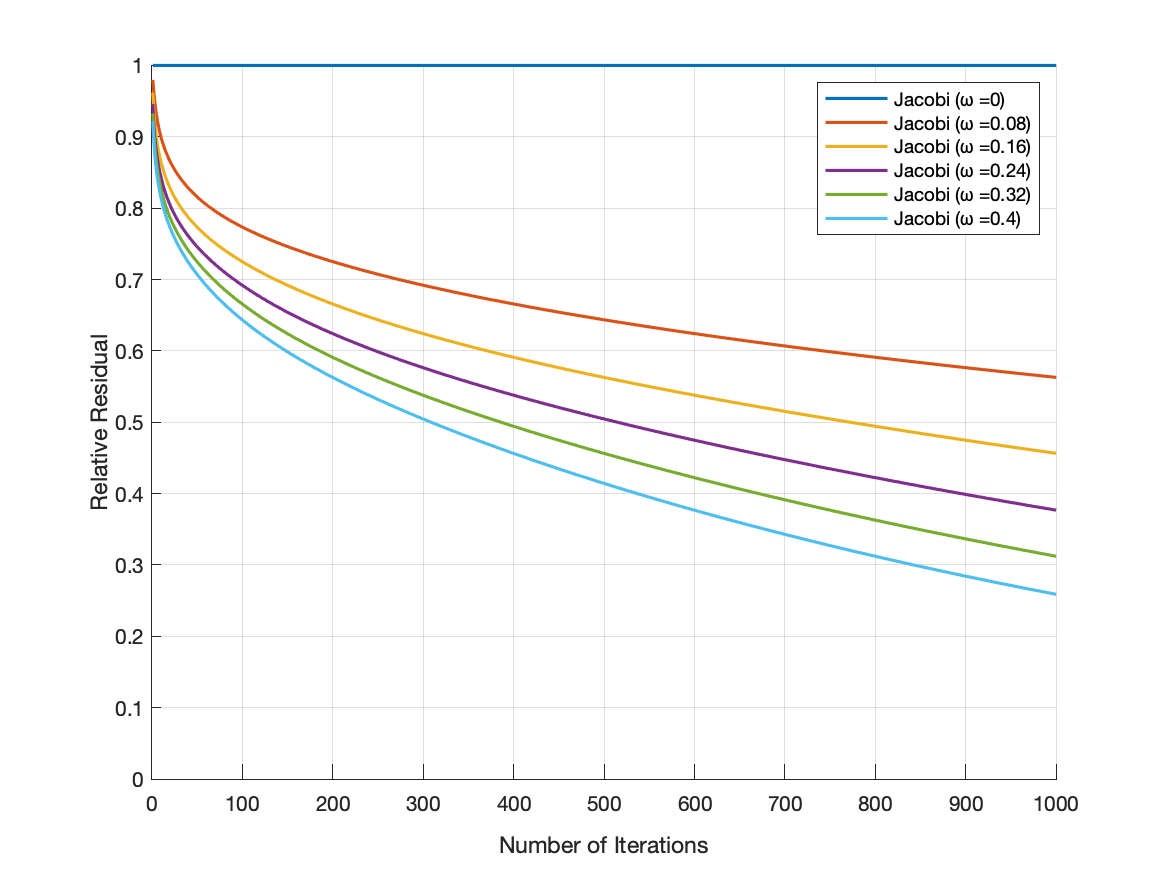
\includegraphics[width=\textwidth]{archbridge_tiny_jacobi_relres_vs_iters}
    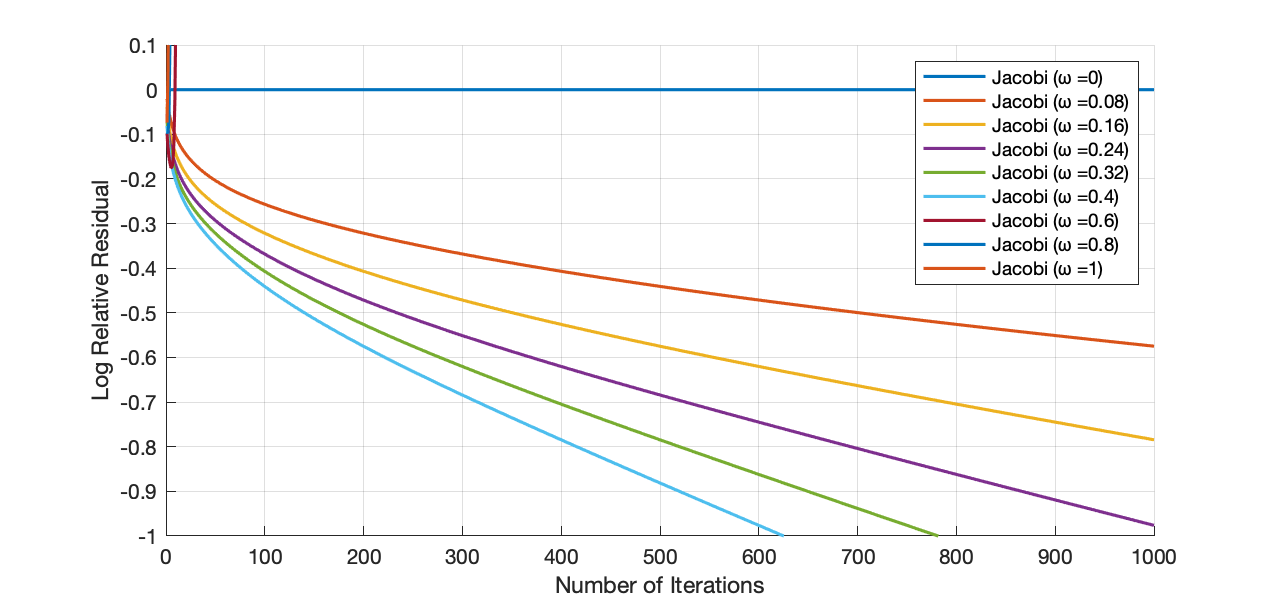
\includegraphics[width=\textwidth]{archbridge_tiny_jacobi_logrelres_vs_iters_full}
    \caption{\label{fig:1} $\omega$-Jacobi's relative residual (top) and log relative residual (bottom) plotted as a function of number of iterations. Each line represent Jacobi's Method with different weights}
\end{center}
\end{figure}

\begin{figure}[!htbp]
    \begin{center}
        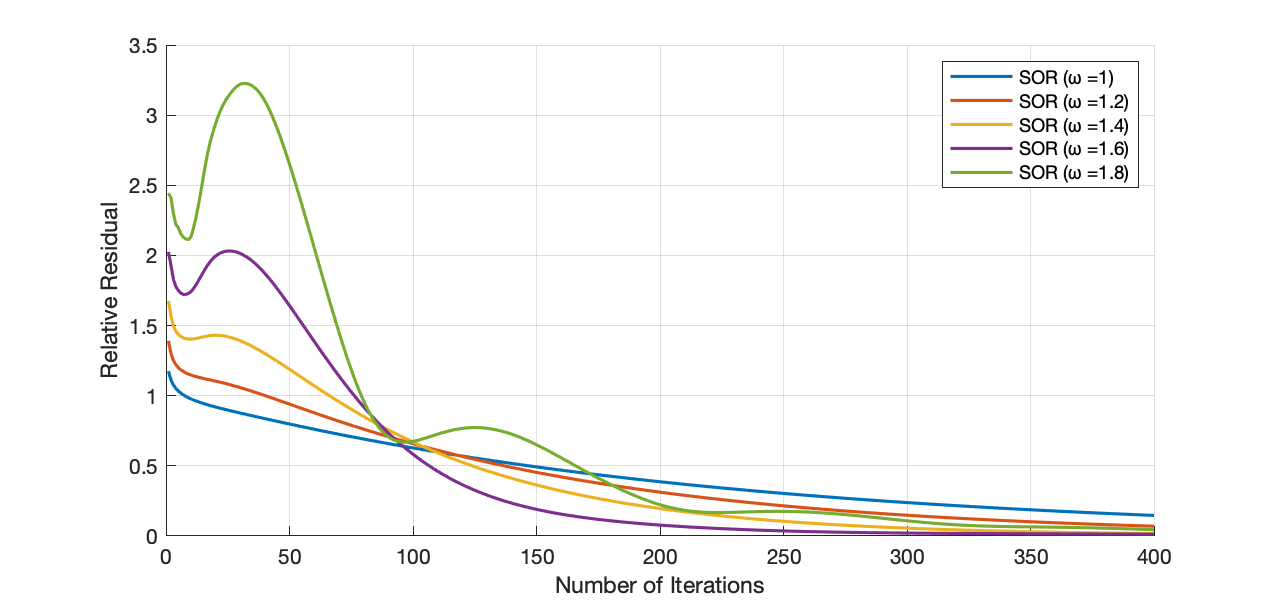
\includegraphics[width=\textwidth]{archbridge_tiny_sor_relres_vs_iters}
        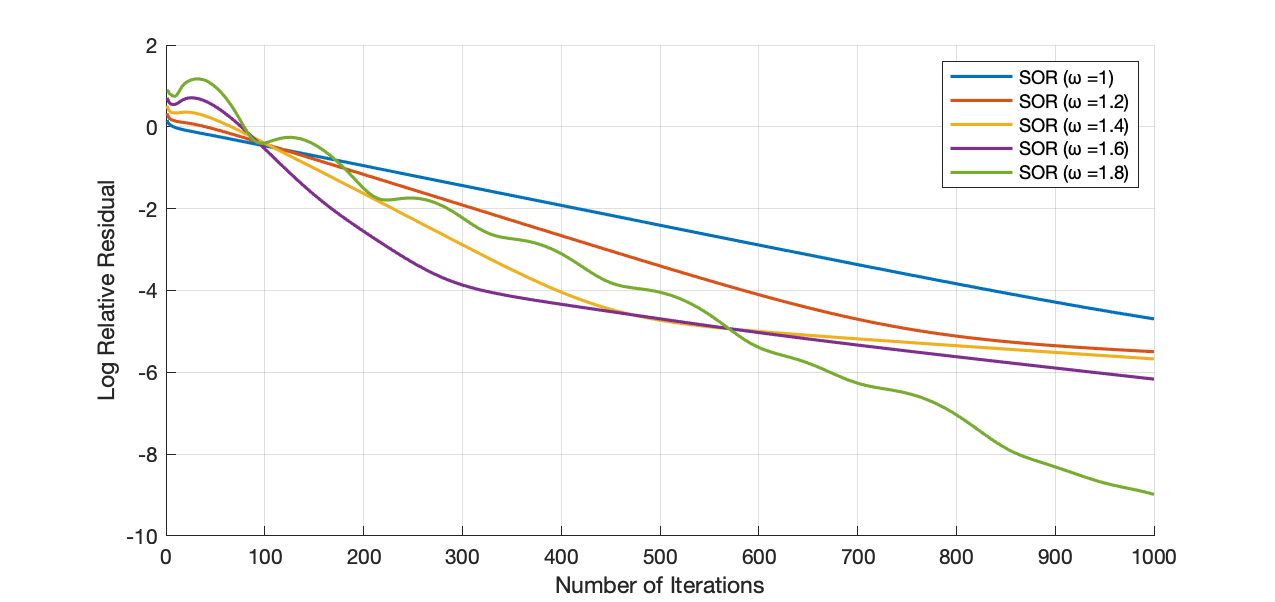
\includegraphics[width=\textwidth]{archbridge_tiny_sor_logrelres_vs_iters}
        \caption{\label{fig:2} SOR's relative residual (top) and log relative residual (bottom) plotted as a function of number of iterations. Each line represent SOR iteration with different weights}
    \end{center}
\end{figure}


\subsection{Approximate Error}

We define error at $k$-th iteration to be, 
\[
    \be^{(k)} = \tilde{\bx} - \bx^{(k)}
\]
where $\tilde{\bx}$ is the real solution of the system. Although $\tilde{\bx}$ is not known, we consider solution resulting from direct LDL/Cholesky solver (\texttt{mldivide}) as the ground truth, and use it in place of $\tilde{\bx}$ to determine an estimate of true error at each iteration. In Figure~\ref{fig:3}, we quantified and compared the performance of $\omega$-Jacobi ($\omega=0.4$) and SOR ($\omega=1.6$) by computing the error norm $\norm{\be}$. We observed that SOR, with a good choice of $\omega$, is much superior to $\omega$-Jacobi.

\begin{figure}[!htbp]
    \begin{center}
        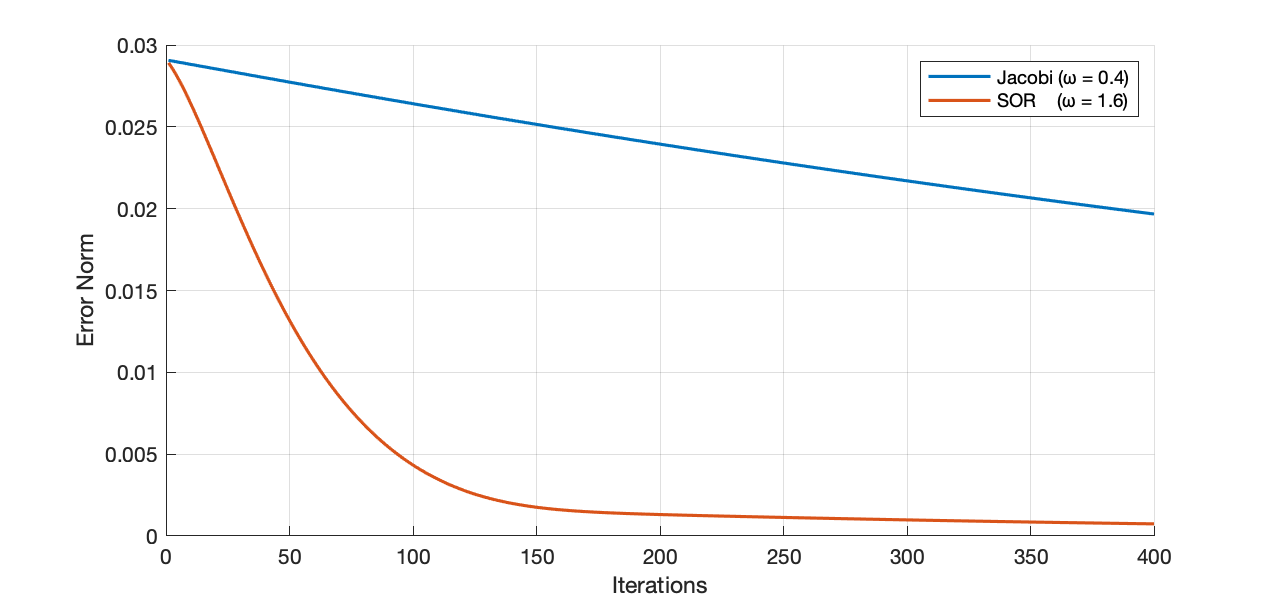
\includegraphics[width=\textwidth]{archbridge_tiny_errornorm.png}
        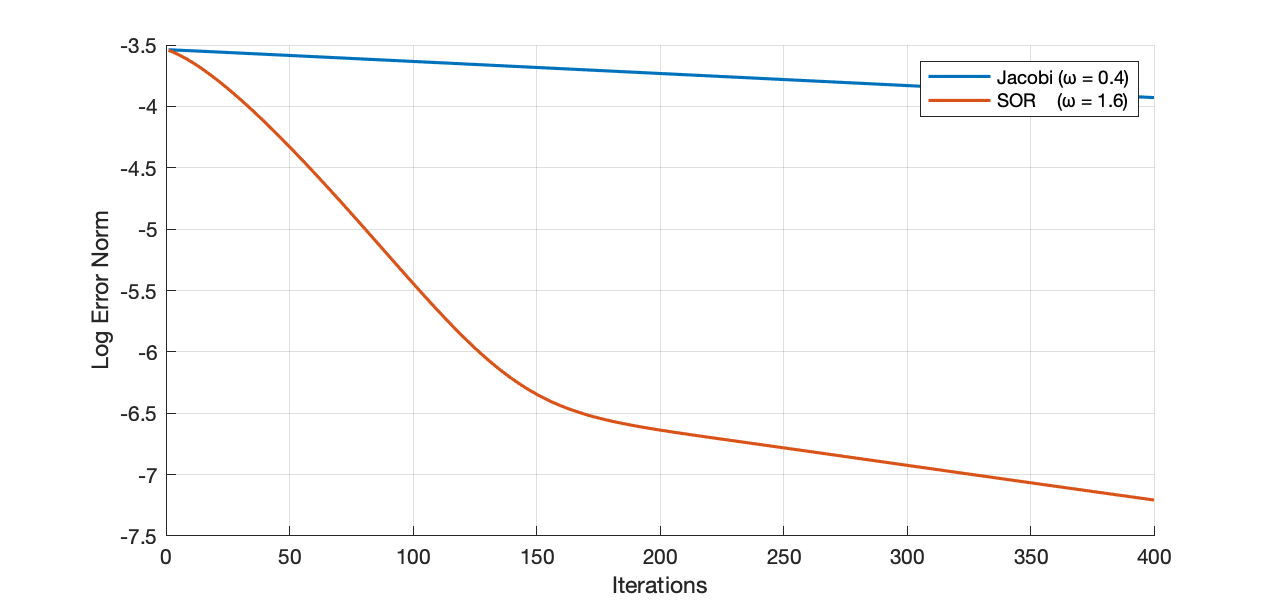
\includegraphics[width=\textwidth]{archbridge_tiny_logerrornorm.png}
        \caption{\label{fig:3} Error (top) and log error (bottom) plotted as a function of number of iterations for different iterative methods}
    \end{center}
\end{figure}

\subsection{Visualizing Stress On Tetrahedron}

Ultimately, we are interested in getting an idea of how few iterations are needed to create a \textit{sensible} visualization of the effective stress field. By \textit{sensible}, we meant that the viewer should be able to get a rough idea of the distribution of the effective stress field, minor local variations can be easily dismissed as long as the global trend is captured with the help of the approximate solutions generated by iterative methods. In Figure~\ref{fig:4}, we plotted the gold standard effective stress field solved using matlab's \texttt{mldivide} solver. 
\begin{figure}[!htbp]
    \begin{center}
        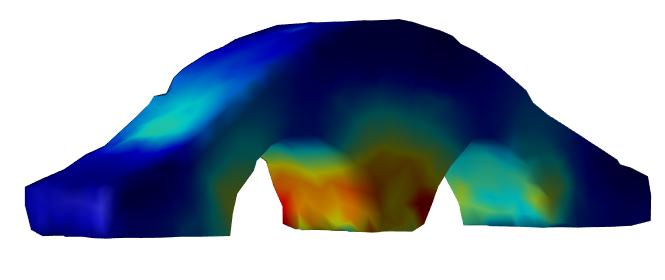
\includegraphics[width=3in]{goldstandard_vm/resized/archbridge_tiny_goldstandard}
        \caption{\label{fig:4} von Minses' effective stress field solved using \texttt{mldivide}}
    \end{center}
\end{figure}
In Figure~\ref{fig:5}, we visualized the effective stress field generated using $\omega$-Jacobi ($\omega=0.4$) and SOR ($\omega=1.6$). Qualitatively, visualization generated using SOR method starting at iteration 200 looks almost indistinguishable from the gold standard., whereas similar observations could be made for $\omega$-Jacobi starting at iteration 500. This suggests that a relative residual of 0.1, resulting in an approximate erorr norm of 0.001, is a \textit{good enough} stopping criterion to guarantee a \textit{sensible} visualization on this particular mesh.
\begin{figure}[!htbp]
    \begin{center}
        $k=1$
        \quad
        \begin{subfigure}[b]{0.4\textwidth}
            \centering
            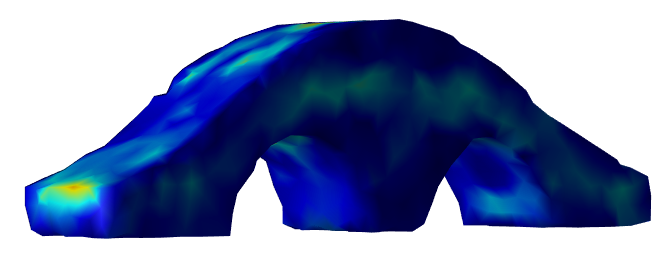
\includegraphics[width=\textwidth]{jacopt_vm/resized/archbridge_tiny_1}
        \end{subfigure}
        \begin{subfigure}[b]{0.4\textwidth}
            \centering
            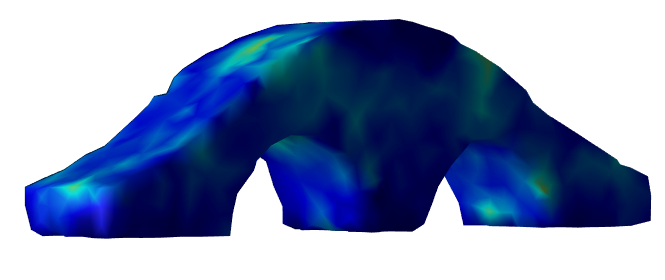
\includegraphics[width=\textwidth]{soropt_vm/resized/archbridge_tiny_1}
        \end{subfigure}\\ 

        $k=50$
        \quad
        \begin{subfigure}[b]{0.4\textwidth}
            \centering
            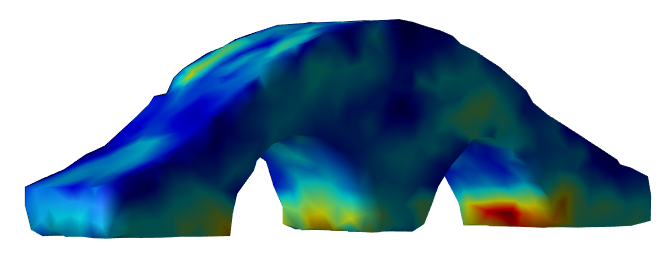
\includegraphics[width=\textwidth]{jacopt_vm/resized/archbridge_tiny_51}
        \end{subfigure}
        \begin{subfigure}[b]{0.4\textwidth}
            \centering
            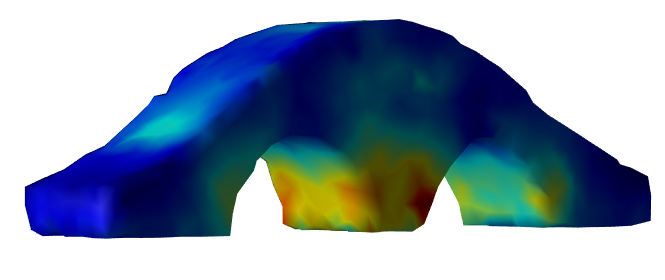
\includegraphics[width=\textwidth]{soropt_vm/resized/archbridge_tiny_51}
        \end{subfigure}\\ 

        $k=100$
        \quad
        \begin{subfigure}[b]{0.4\textwidth}
            \centering
            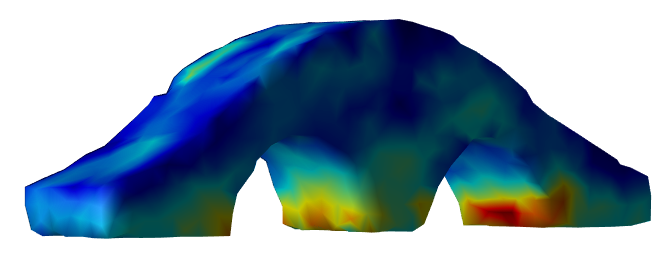
\includegraphics[width=\textwidth]{jacopt_vm/resized/archbridge_tiny_100}
        \end{subfigure}
        \begin{subfigure}[b]{0.4\textwidth}
            \centering
            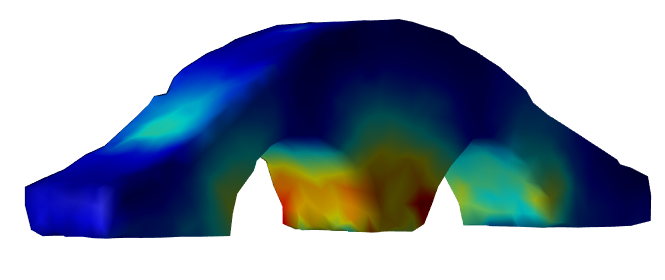
\includegraphics[width=\textwidth]{soropt_vm/resized/archbridge_tiny_100}
        \end{subfigure}\\ 


        $k=200$
        \quad
        \begin{subfigure}[b]{0.4\textwidth}
            \centering
            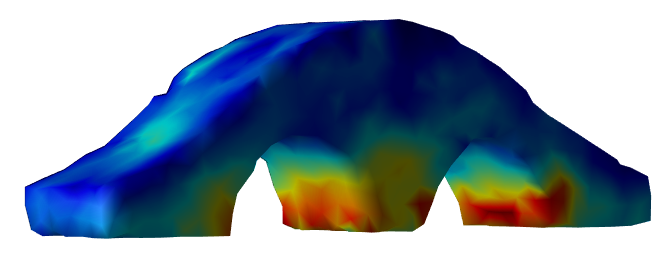
\includegraphics[width=\textwidth]{jacopt_vm/resized/archbridge_tiny_200}
        \end{subfigure}
        \begin{subfigure}[b]{0.4\textwidth}
            \centering
            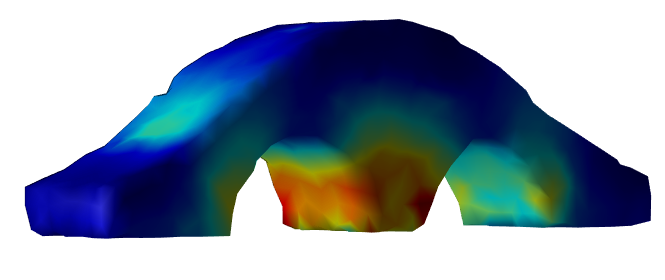
\includegraphics[width=\textwidth]{soropt_vm/resized/archbridge_tiny_200}
        \end{subfigure}\\ 


        $k=500$
        \quad
        \begin{subfigure}[b]{0.4\textwidth}
            \centering
            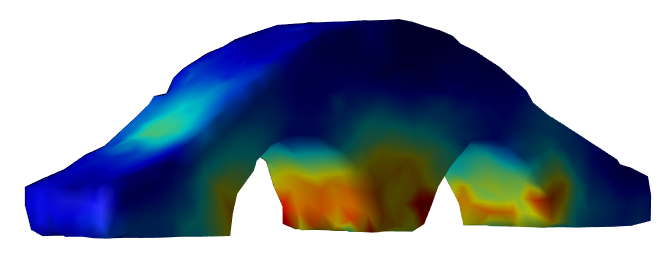
\includegraphics[width=\textwidth]{jacopt_vm/resized/archbridge_tiny_500}
        \end{subfigure}
        \begin{subfigure}[b]{0.4\textwidth}
            \centering
            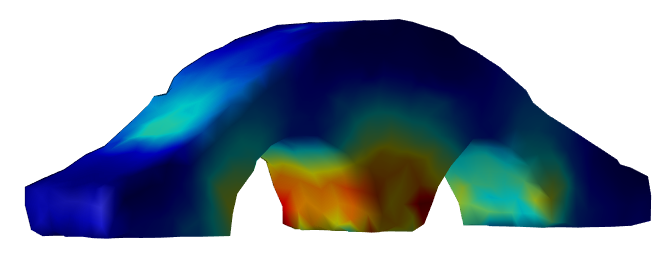
\includegraphics[width=\textwidth]{soropt_vm/resized/archbridge_tiny_500}
        \end{subfigure}\\ 


        $k=1000$
        \quad
        \begin{subfigure}[b]{0.4\textwidth}
            \centering
            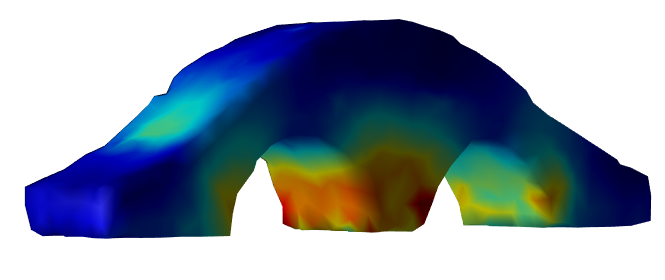
\includegraphics[width=\textwidth]{jacopt_vm/resized/archbridge_tiny_1000}
        \end{subfigure}
        \begin{subfigure}[b]{0.4\textwidth}
            \centering
            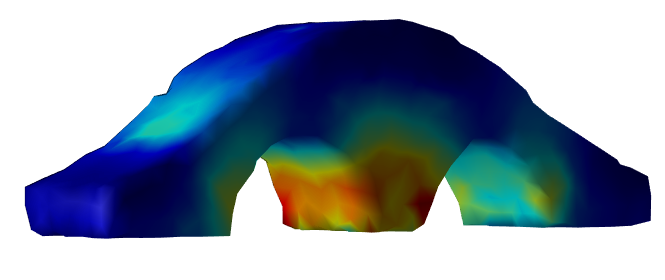
\includegraphics[width=\textwidth]{soropt_vm/resized/archbridge_tiny_1000}
        \end{subfigure}\\ 
        \caption{\label{fig:5} von Mises' effective stress field generated from $\omega$-Jacobi ($\omega=0.4$) and SOR ($\omega=1.6$) at iterations $k=1,50,100,200,500,1000$}
    \end{center}
\end{figure}

\section{Discussion \& Conclusion}

We have demonstrated that even with the simpliest iterative method, we can achieve undistinguishable stress field visualization from direct solvers, in a few number of iterations. This is all achieved without exploring more sophisticated iterative methods like conjugated gradient, multigrid, etc. or hand-tuned preconditioners. Additionally, we have demonstrated how we could save memory and time cost associated with assembly of stiffness matrices $\bK$ with the help of regular hexahedron element. To conclude, matrix-free iterative methods over regular hexahedron elements have great potential in real-time linear elasticity simulation, especially for visualization purposes where \textit{good enough} approximate solutions can generate \textit{sensible} visualizations.
However, there are complications along the way. For example, we need to experimentally determine the optimal parameter $\omega$ for both iterative method tested. Theories for finding optimal parameters have assumptions that linear leasticity simulation cannot make; So we had to resort to finding a good choice of $\omega$ experimentally via a simple grid search. Another complication comes with the use of trilinear interpolation to map stress field back from voxel grids to the tetrahedron mesh. We noticed obvious artifacts when the resolution of the voxel grids is coarse.

\section{Future Directions}

Given the limited amount of time to undertake this project, there is still so much we had not have enough time to look at. A short list of to-dos is as follows,
\begin{enumerate}
    \item Explore other linear solvers that is more robust and efficient, i.e. conjugate gradient, multigrid
    \item Explore preconditioner that helps with solving linear elasticity problem faster
    \item Explore different interpolation schemes for mapping stress field back from voxel grids to tetrahedron mesh
    \item Implement linear solvers on GPU for real-time simulation
\end{enumerate}


\newpage
\printbibliography

\end{document}
